\chapter{Teoretyczne podstawy integracji mikroserwisów}
\section{Wstęp}
W systemach rozproszonych zbudowanych z kilkudziesięciu lub nawet kilku tysięcy mikroserwisów komunikacja pomiędzy nimi jest jednym z najważniejszych aspektów. Od poprawnego zaprojektowania API oraz doboru właściwych technologii zależy, czy system będzie elastyczny jeśli chodzi o integrację z zewnętrznymi odbiorcami oraz wykorzysta większość zalet jakie oferują mikroserwisy.
\section{Technologie oraz protokoły używane do komunikacji pomiędzy mikroserwisami}
\subsection{HTTP oraz HTTP/2}
Z początkiem lat dziewięćdziesiątych XX wieku na skraju powstania ogólnoświatowego medium informacji jakim jest internet opracowano prosty protokół \textbf{HTTP (\textit{(ang. Hypertext Transfer Protocol)}}. Będąc umiejscowionym w najwyższej warstwie (aplikacji) modelu TCP/IP służy do obsługi żądań oraz odpowiedzi w relacji klient-serwer \cite{gourley2002http}. Każde żądanie oraz odpowiedź mają postać wiadomości, która jest zapisana w postaci tekstu przez co jest prosta w odczycie przez człowieka. Wiadomości składają się z następujących elementów:
\begin{itemize}
    \item  \textbf{Linia początkowa}-podczas żądania w tej linii określa się z jakiej metody HTTP chce się skorzystać (m.in.\ GET, POST, PUT, DELETE) oraz wersję protokołu (najczęściej HTTP/1.1). Odpowiedź zawiera wersję protokołu oraz kod statusu odpowiedzi (np. 200, 404, 500)
    \item  \textbf{Nagłówki HTTP}-nagłówki zawierają dane w postaci \textit{nazwa-nagłówka: wartość-nagłówka}, które określają m.in.\ adres serwera, informacje na temat połączenia czy format danych jakie są akceptowane \cite{gourley2002http}
    \item \textbf{Ciało wiadomości}-opcjonalny element wiadomości zwierający dane w dowolnym formacie uzgodnionym w nagłówku 
\end{itemize}
Protokół HTTP jest bezstanowy co oznacza, że serwer nie może zapisać stanu żądania od klienta i użyć go gdy przyjdzie następne. Każdy zasób sieciowy do którego odwołuje się klient jest identyfikowany za pomocą \textbf{URI \textit{(ang. Uniform Resource Identifier)}} \cite{berners2014rfc}. Jest to unikalny identyfikator składający się z sekwencji znaków będący referencją do konkretnego zasobu umieszczonego na serwerze HTTP.\@ Prostota oraz całkiem jawny sposób przesyłania wiadomości powoduje, że protokół HTTP jest całkowicie niezabezpieczony umożliwiając tym samym proste przechwycenie wiadomości. Panaceum na tą dolegliwość jest rozszerzana wersja \textbf{HTTPS \textit{(ang. Hypertext Transfer Protocol Secure)}}. Wiadomości przenoszone za pomocą tego protokołu są dodatkowa szyfrowane za pomocą certyfikatów SSL.\@
\par Przez lata HTTP/1.1 był najbardziej popularnym protokołem używanym w sieci internetowej oraz podczas korzystania z usług sieciowych. Jednak zwiększające zasoby na stronach internetowych powodowały, że do wczytania wszystkich treści potrzeba setek żądań. Powoduje to wolniejsze wczytywanie bogatych w treści i multimedia portali. Dlatego w roku 2015 organizacja \textbf{IETF \textit{(Internet Engineering Task Force)}} opracowała standard HTTP/2\cite{belshe2015hypertext}. Jednymi z głównych zmian względem protokołu HTTP/1.1 są:
\begin{enumerate}
    \item Dane przekazywane za pomocą protokołu są zapisane binarnie przez co wielkość wiadomości ulega znacznemu zmniejszeniu oraz zwiększa wydajność parsowania danych, 
    \item Transmisja danych odbywa się za pomocą jednego połączenia TCP eliminując tym samym obciążenie serwera związane z ciągłym odpytywaniem przez klienta o kolejne zasoby \cite{ludin2017learninghmultiplex},
    \begin{figure}[h]
        \caption{Porównanie działania połącznia protokołu HTTP/1.1 oraz HTTP/2}
        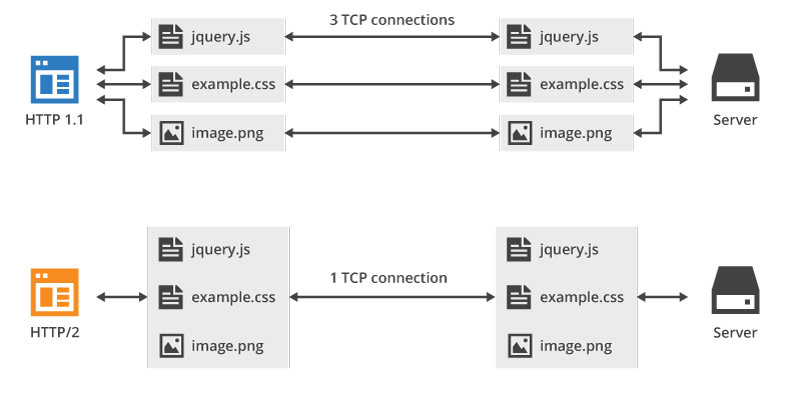
\includegraphics[width=\textwidth]{http2_connection}
        \centering
    \end{figure}
    \item Klient ma możliwość ustawienia priorytetu dla zwracanych przez serwer danych poprzez ustawianie wag dla każdego z elementów strony \cite{ludin2017learninghmultiplex},
    \item  Nagłówki wiadomości są kompresowane. Do serwera wysyłane są tylko części unikalne. Cała reszta nagłówka jest odrzucana \cite{ludin2017learninghmultiplex},
    \item Serwer ma możliwość wypychania danych zanim klient o nie zapyta \cite{ludin2017learninghmultiplex}. 
\end{enumerate}  
\subsection{REST}
Pojęcie REST (\textit{(Representational State Transfer)}) pojawiło się w roku 2000 w pracy doktorskiej Roya Fieldinga \cite{thomas2000architectural} i oznacza styl architektoniczny dla systemów rozproszonych. Usługa REST będąc oparta na protokole HTTP wykorzystuje udostępniane przez niego metody (\textit{GET, POST, PUT, DELETE}) do manipulacji na zdalnych zasobach do których dostęp jest wskazywany przy użyciu unikalnych wzorców identyfikatorów URI (\textit{Uniform Resource Identifier}). Metody te odwzorowują funkcje \textbf{create (utwórz)}, \textbf{read (odczytaj)}, \textbf{update (aktualizuj)} oraz \textbf{delete (usuń)} znane pod kryptonimem \textit{CRUD}.\@
W swojej pracy Fielding nie tylko przedstawił definicję usługi REST, ale także zapisał wiele wytycznych, które służyły przyszłym projektantom przy budowie swoich serwisów. Zbiór tych reguł wraz z późniejszymi pracami rozwijającymi tą dziedzinę kryje się pod pojęciem \textbf{HATEOAS (\textit{Hypermedia As The Engine Of Application State})}. Interfejs API, który jest zbudowany z wykorzystaniem zasad HATEOAS wymaga od klienta wykrycia funkcji jakie udostępnia. Klient który chciałby wykorzystać interfejs musi wykonać zapytanie GET na głównym identyfikatorze URI. W ten sposób otrzyma szczegółową listę identyfikatorów, które będą mogły zostać wykorzystane do obsługi innych operacji. Identyfikatory te nie mogą być przechowywane przez klienta wymuszając dynamiczną analizę. Wymaga to od programisty po stronie klienta zaimplementowanie mechanizmów, które będą umożliwiały dostosowanie się do zmian po stronie serwera. Reguła ta umożliwia projektantom interfejsów dowolną ich modyfikację bez obawy, że po stronie klienta wystąpią problemy z ich użytkowaniem. Pomimo faktu, iż rozwiązanie to przekłada się na lepszą skalowalność oraz rozszerzalność klientów oraz serwerów upraszczało pracę tylko projektantom po stronie serwera. Programiści po stronie klienta musieli pilnować, aby nie umieścić identyfikatora na stałe co przy rosnącym poziome skomplikowania API prowadziło do wielu pomyłek. Tym samym narodził się bardziej pragmatyczny wariant REST. Pozostawiono najlepsze cechy starszej specyfikacji wprowadzając znaczne ułatwienia dla programistów po stronie klienta.
Poniższe zasady mają za zadanie uporządkować standard REST tak, aby ułatwić integrację usług \cite{jacobson2015interfejsapi}:
\begin{itemize}
    \item działania na pojedynczych obiektach powinny korzystać z wszystkich dostępnych metod udostępnionych przez HTTP.\@ Do tej pory najczęściej wykorzystywana była metoda PUT,
    \item należy stosować kody powrotu dla odpowiedzi serwera,
    \item programista po stronie klienta powinien jakiego formatu danych ma się spodziewać wywołując metodę,
    \item każda kolejna wersja API powinna zawierać w identyfikatorze URI numer wersji,
    \item identyfikatory URI powinny być zaprojektowane według ustalonego wzorca,
    \item nagłówki HTTP powinny zawierać jedynie wymagane informacje
\end{itemize}
\begin{table}[h]
    \begin{center}
        \caption{Przykład użycia metod HTTP wraz z opisem operacji oraz identyfikatorami URI}
        \hspace*{-1cm}
        \begin{tabular}{|M|c|L|}
            \toprule
            \textbf{Operacja}               & \textbf{Metoda} & \textbf{Identyfikator URI}                                      \\
            \midrule
            Umieszczenie produktu w koszyku & POST            & \url{http://api.v1.eshop/bucket/bucketName}                     \\
            \midrule
            Wyświetlenie zawartości koszyka & GET             & \url{http://api.v1.eshop/bucket/bucketName}                     \\
            \midrule
            Pobranie produktu z koszyka     & GET             & \url{http://api.v1.eshop/bucket/bucketName/product/productName} \\
            \midrule
            Zastępowanie produktu w koszyku & PUT             & \url{http://api.v1.eshop/bucket/bucketName/product/productName} \\
            \midrule
            Usuwanie produktu z koszyka     & DELETE          & \url{http://api.v1.eshop/bucket/bucketName/product/productName} \\
            \midrule
            Usuwanie całego koszyka         & DELETE          & \url{http://api.v1.eshop/bucket/bucketName}                     \\
            \bottomrule
        \end{tabular}
        \hspace*{-1cm}
    \end{center}
\end{table}
W swojej pierwotnej formie REST był zaprojektowany do wymiany informacji przy użyciu protokołu XML.\@ Format ten posiada olbrzymie możliwości jeśli bierze się pod uwagę tworzenie skomplikowanych obiektów z zagwarantowaną spójnością. Biorąc pod uwagę, że usługi REST charakteryzują się prostotą oraz lekkością pobieranie znacznych ilości danych w postaci XML stało się niewygodne. Godnym następcą okazał się format \textbf{JSON \textit{JavaScript Object Notation}}. Format ten został opracowany przez Douglasa Crockforda, który wykorzystał elementy języka JavaScript budując tym samym lekki oraz prosty język definicji danych. Największą zaletą formatu JSON jest możliwości translacji bezpośrednio w używanych językach programowania, bez konieczności konwersji na obiekty tak jak ma to miejsce w przypadku formatu XML.\@ Format XML wymusza również implementację mechanizmów analizowania składni ze względu na implementację atrybutów, przestrzeni nazw lub wariantów kodowania tekstu.
\begin{lstlisting}[language=xml, caption=Dane zapisane w formacie XML]
<?xml version="1.0" encoding="iso-8859-1"?>
<users>
  <user>
    <firstname>Paul</firstname>
    <surname>Sajnog</surname>
    <address>Wolczanska 12</address>
    <city>Lodz</city>
    <country>Poland</country>
    <contact>
      <phone>666 777 000</phone>
      <email>167686@edu.p.lodz.pl</email>
    </contact>
  </user>
</users>
\end{lstlisting}
\newpage
\begin{lstlisting}[caption=Dane zapisane w formacie JSON]
{
    "users": {
        "user": {
            "firstname": "Paul",
            "surname": "Sajnog",
            "address": "Wolczanska 12",
            "city": "Lodz",
            "country": "Poland",
            "contact": {
                "phone": "666 777 000",
                "email": "167686@edu.p.lodz.pl"
            }
        }
    }
}
    \end{lstlisting}
\subsection{RPC}
Koncepcja RPC (\textit{Remote Procedure Call}) jest znacznie starsza niż wcześniej przedstawiona REST.\@ Już w roku 1981 dokładnie została opisana w publikacji inżynierów pracujących w laboratoriach Xerox \cite{nelson1981remote}. Architektura takiego rozwiązania opiera się na modelu klient-serwer. W momencie gdy zachodzi potrzeba wywołania zdalnej program kliencki przekazuje parametry do metody lokalnej tak jak się to odbywa w przypadku normalnych aplikacji. W tym momencie bez jakiejkolwiek wiedzy po stronie klienta na temat połącznia sieciowego środowisko uruchomieniowe RPC przekazuje dane do usługi uruchomionej po stronie serwera, który znajduje się w innej adresacji sieciowej. Gdy już się zakończy przetwarzanie żądania serwer zwraca tą samą drogą odpowiedź z wynikiem. Cały proces przebiega w sposób synchroniczny więc klient oczekuje do czasu, aż serwer zwróci mu odpowiedź. Główną ideą RPC jest ukrywanie wszelkich informacji na temat sieciowej warstwy transportowej oraz mechanizmów serializacji oraz deserializacji przesyłanych danych. Ma to na celu odciążyć programistów, którzy nie muszą już implementować kodu odpowiedzialnego za przygotowanie danych do wysyłki oraz podejmowania decyzji o doborze warstwy transportowej.
\begin{figure}[h!]
    \caption{Diagram sekwencji przedstawiający przebieg wywołania zdalnej metody}
    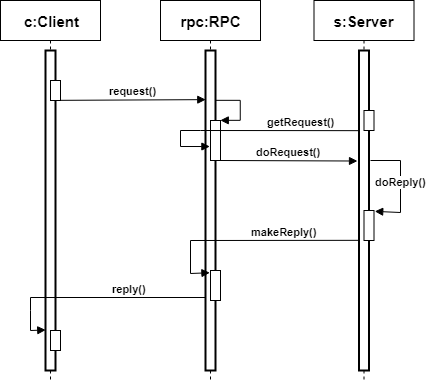
\includegraphics[width=\textwidth]{rpc_dig_sekw}
    \centering
\end{figure} 
\par W większości technologii opartych na protokole RPC proces tworzenia usługi RPC rozpoczyna się od zdefiniowania udostępnionych interfejsów w specjalnym języku \textbf{IDL \textit{Interface Description Language}}. W przypadku technologii XML-RPC oraz JSON-RPC funkcjonalność tą można uzyskać za pomocą dodatkowych bibliotek. Język ten nie ma ustalonego standardu dla wszystkich rozwiązań dostępnych na rynku. W zależności od użytej technologii różni się on składnią oraz definiowaniem konkretnych abstrakcji danych używanych w procesie wymiany pomiędzy serwerem oraz klientem. Następnie z tak przygotowanych definicji wygenerowane zostają specjalne części kodu(\textit{ang. stubs}) osobno dla klienta i serwera. Każda ze stron implementuje wygenerowany kod. Po stronie serwera pozostaje dodać odpowiednią logikę, która zajmuje się przetwarzaniem odebranych danych. Różne rozwiązania stosują różne formaty danych w niektórych wypadkach jest to format binarny (Java RMI, Apache Thrift, gRPC) w innych XML lub JSON (SOAP, XML-RPC, JSON-RPC). Za warstwę transportową może posłużyć protokół TCP, UDP lub HTTP\@.
\begin{figure}[h!]
    \caption{Przykład implementacji usługi RPC}
    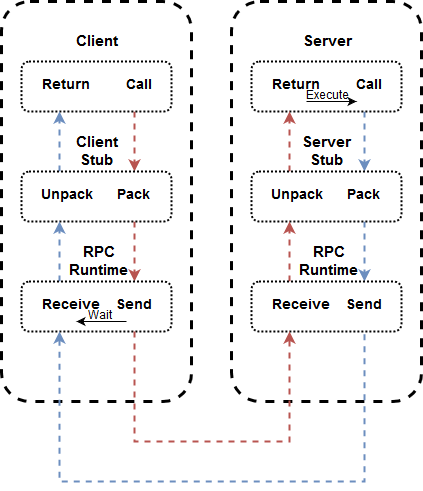
\includegraphics[width=\textwidth]{rpc}
    \centering
\end{figure}
\section{Komunikacja synchroniczna i asynchroniczna}
Gdy projektant rozpoczyna planowanie wdrożenia architektury mikroserwisowej musi podjąć decyzję, czy komunikacja pomiędzy mikroserwisami ma być synchroniczna, czy asynchroniczna. Decyzja ta ma olbrzymi wpływ na to jak będzie w przyszłości zachowywał się cały system. W podejściu synchronicznym klient po wysłaniu żądania, będzie oczekiwał na odpowiedź serwera. Asynchroniczna komunikacja umożliwia klientowi wykonywanie innych działań po wysłaniu żądania. Oba podejścia niejako wymuszają różne modele współpracy. Synchroniczny model komunikacji jest dużo łatwiejszy do zamodelowania jednak nie sprawdzi się w przypadku, gdy zadania do wykonania są długotrwałe lub gdy oczekuje się niewielkich opóźnień ze względu na swoją blokującą naturę. Różne tryby komunikacji mają wpływ na styl współpracy między mikroserwisami. Architektura oparta na stylu żądanie-odpowiedź działa w klasyczny sposób, gdzie to klient inicjuje żądanie i czeka na odpowiedź serwera. Innym stylem jest architektura oparta na zdarzeniach. W tym wypadku klient generuje zdarzenie, które zostaje zarejestrowane przez magistralę zdarzeń (np. RabbitMQ), a następnie przekierowane do odpowiedniej usługi. Tutaj klient nie jest powiadamiany, gdzie trafi jego żądanie. 
\subsection{Orkiestracja i choreografia}
W momencie, gdy procesy biznesowe wychodzą poza granicę pojedynczej usługi pojawia się problem zarządzania nimi. Szczególnie podatne na te zagrożenia są mikroserwisy. Aby temu zaradzić zaproponowano dwa różne podejścia. W pierwszym specjalnie do tego powołany koordynator aranżuje wysyłanie wielu żądań do odpowiednich usług oczekując na odpowiedź. Wzorzec oparty na choreografii pozwala usłudze klienckiej na wyemitowanie danego zdarzenia, które trafia do magistrali zdarzeń. Tam jest subskrybowane przez każdy dołączony serwis, który wykonuje swoje działania gdy zachodzi taka potrzeba. Pierwsze podejście opiera swoją komunikację na wywołaniach synchronicznych z każdym serwisem, który jest zaangażowany w przetwarzanie żądania. Dodatkowo zabierana jest w pewien sposób autonomiczność każdego z mikroserwisów, które są uzależnione od poleceń koordynatora. Podejście oparte na choreografii pozwala działać w sposób asynchroniczny, gdyż każda usługa działa niezależnie wykonując swoje zadanie.
\begin{figure}[hbt!]
    \caption{Porównanie grafów zależności dla orkiestracji oraz choreografii w architekturze mikroserwisowej}
    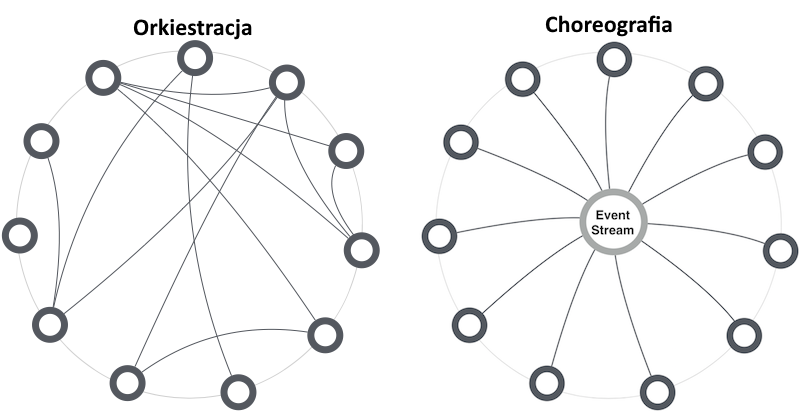
\includegraphics[width=\textwidth]{orchea_choreo}
    \centering
\end{figure}